\subsection{Introduction}

Variational Autoencoders (VAEs) are latent-variable generative models that
learn a probabilistic mapping between observed data $x$ and a lower-dimensional
latent code $z$, optimized via a tractable lower bound on the data
log-likelihood (the ELBO) rather than the intractable marginal likelihood
$p(x)=\int p(x|z)p(z)\,dz$ directly. Unlike a plain autoencoder, a VAE
regularizes its latent code toward a fixed prior $p(z)=\mathcal{N}(0,I)$,
which is what allows it to be used generatively: sampling $z$ from the prior
and decoding it should produce plausible new data, not just reconstructions
of inputs it has already seen.

This section implements a basic MLP-based VAE for MNIST, then evaluates what
the model has actually learned along three axes -- the organization of its
latent space, the fidelity of its reconstructions, and the quality of images
generated purely from the prior -- compares two latent dimensionalities
($d=128$ and $d=32$) against each other, and compares the design and results
against Doersch's (2016) reference tutorial and implementation.

\subsection{Methodology}

\subsubsection{Model Architecture}

The encoder is a multi-layer perceptron $784 \to 512 \to 256 \to (\mu,\log\sigma^2)$:
two shared hidden layers with ReLU activations feed two separate linear
output heads, one producing the approximate posterior's mean
$\mu_\phi(x) \in \mathbb{R}^{d}$, the other its log-variance
$\log\sigma^2_\phi(x) \in \mathbb{R}^{d}$. Both heads are unconstrained
linear outputs -- critically, the log-variance parameterization means no
activation function is required to guarantee a valid (positive) variance,
since $\sigma^2 = \exp(\log\sigma^2)$ is positive for any real-valued input.
The decoder mirrors the encoder, $d \to 256 \to 512 \to 784$, with a final
sigmoid activation producing per-pixel Bernoulli probabilities in $[0,1]$,
matching MNIST's normalized pixel range. Two latent dimensionalities are
trained under an otherwise identical protocol: the primary configuration,
$d=128$, and a second configuration, $d=32$, trained to directly test
Doersch's claim that VAE behavior is largely insensitive to latent
dimensionality across a broad middle range.

\subsubsection{Reparameterization and Loss Formulation}

To backpropagate through the stochastic sampling step $z \sim q_\phi(z|x)$,
we use the reparameterization trick: sample $\epsilon \sim \mathcal{N}(0,I)$
independently of any trainable parameter, and compute
\[
  z = \mu_\phi(x) + \sigma_\phi(x) \odot \epsilon, \qquad
  \sigma_\phi(x) = \exp\!\left(\tfrac{1}{2}\log\sigma_\phi^2(x)\right).
\]
This pushes all randomness into $\epsilon$, so gradients can flow from the
reconstruction loss back through $\mu_\phi$ and $\sigma_\phi$ into the
encoder's weights.

The training objective is the negative ELBO, decomposed into a
reconstruction term and a KL-regularization term:
\[
  \mathcal{L}(x) = \underbrace{-\sum_i\big[x_i\log\hat{x}_i+(1-x_i)\log(1-\hat{x}_i)\big]}_{\text{reconstruction (binary cross-entropy)}}
  \;+\; \underbrace{D_{KL}\big(q_\phi(z|x)\,\|\,\mathcal{N}(0,I)\big)}_{\text{KL term}},
\]
with the closed-form Gaussian KL divergence, implemented exactly as
\[
  D_{KL}\big(\mathcal{N}(\mu,\sigma^2)\,\|\,\mathcal{N}(0,I)\big)
  = -\tfrac{1}{2}\sum_{j=1}^{d}\big(1+\log\sigma_j^2-\mu_j^2-\sigma_j^2\big).
\]

\subsubsection{Training Configuration}

Each model is trained on the MNIST training split (50{,}000 train /
10{,}000 validation images, pixel values scaled to $[0,1]$, no further
normalization, since BCE requires targets in $[0,1]$) for 20 epochs using
Adam ($\text{lr}=1\times10^{-3}$) and minibatch SGD with batch size 32.

\subsection{Results}

\subsubsection{Training Dynamics ($d=128$)}

\begin{figure}[t]
\centering
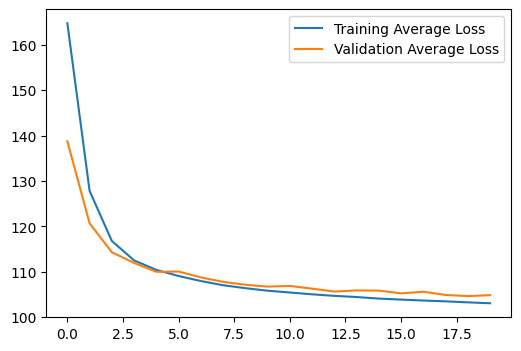
\includegraphics[width=\linewidth]{assets/vae_fig1.png}
\caption{Total loss (reconstruction + KL) over 20 epochs, $d=128$, training and validation.}
\label{fig:vae-loss}
\end{figure}

\begin{figure}[t]
\centering
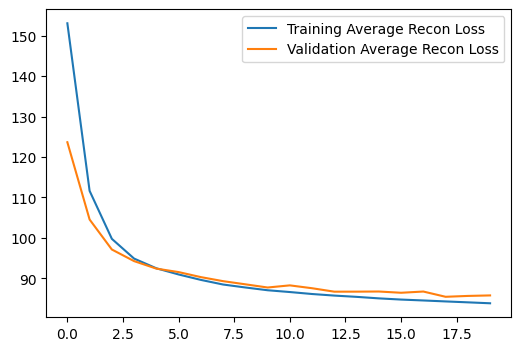
\includegraphics[width=\linewidth]{assets/vae_fig2.png}
\caption{Reconstruction (BCE) loss over training, $d=128$.}
\label{fig:vae-recon-loss}
\end{figure}

\begin{figure}[t]
\centering
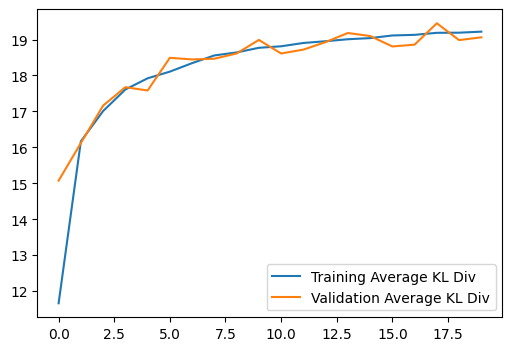
\includegraphics[width=\linewidth]{assets/vae_fig3.png}
\caption{KL divergence over training, $d=128$.}
\label{fig:vae-kl}
\end{figure}

Total loss decreases monotonically from 164.73 to 103.05 (training) over 20
epochs (Figure~\ref{fig:vae-loss}), with validation loss following closely
(138.73 $\to$ 104.83) and no evidence of overfitting at this scale.
Reconstruction loss (Figure~\ref{fig:vae-recon-loss}) falls steadily from
153.07 to 83.83 (training). KL divergence (Figure~\ref{fig:vae-kl}) shows
the opposite trend, rising from 11.66 to 19.22 (training) before
plateauing in the last few epochs: early in training the posterior stays
close to the prior (little information encoded yet); as reconstruction
improves, the encoder must encode increasingly image-specific information,
which costs KL. Final held-out test-set metrics: total loss 104.39,
reconstruction 85.27, KL divergence 19.12 (consistent: $85.27+19.12=104.39$).

\subsubsection{Reconstruction Quality ($d=128$)}

\begin{figure}[t]
\centering
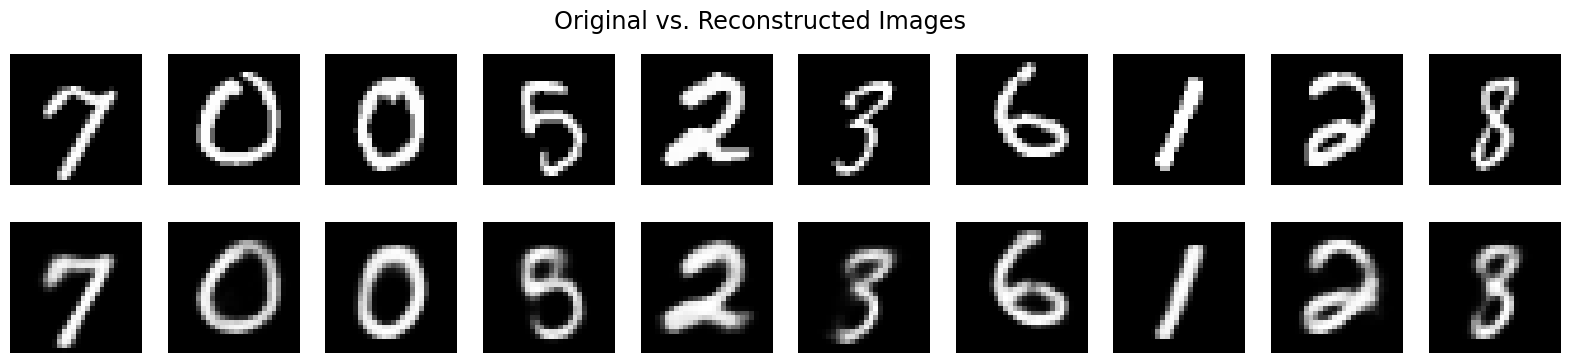
\includegraphics[width=\linewidth]{assets/vae_fig4.png}
\caption{Training-set digits (top row) and their VAE reconstructions (bottom row), $d=128$.}
\label{fig:vae-recon}
\end{figure}

Figure~\ref{fig:vae-recon} shows ten digits (7,0,0,5,2,3,6,1,2,8) and their
reconstructions. Every digit's class identity is preserved; no digit is
reconstructed as a different class. Reconstructions are visibly blurrier
and softer-edged than the originals, most noticeably on the closed loop of
``5'' and the rounded strokes of ``8''.

\subsubsection{Generation of New Samples ($d=128$)}

\begin{figure}[t]
\centering
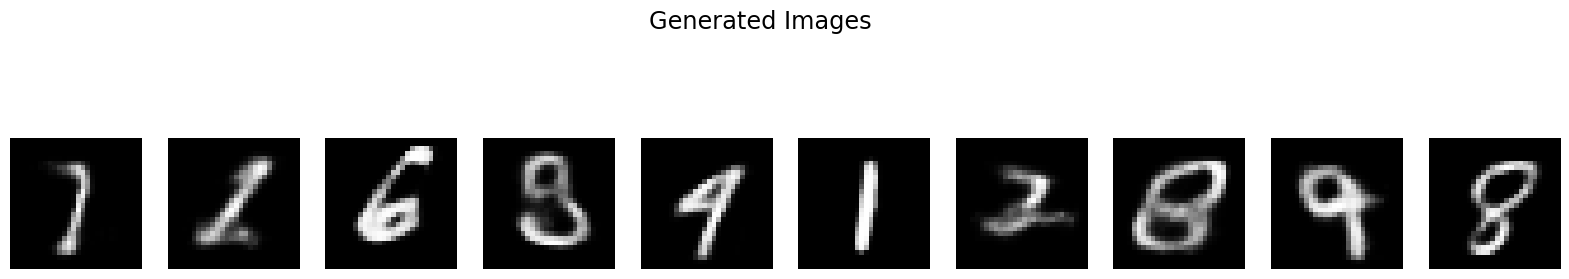
\includegraphics[width=\linewidth]{assets/vae_fig5.png}
\caption{Ten digits generated by decoding $z\sim\mathcal{N}(0,I)$ sampled directly from the prior, $d=128$.}
\label{fig:vae-gen}
\end{figure}

Figure~\ref{fig:vae-gen} shows ten images decoded from $z$ sampled directly
from the prior $\mathcal{N}(0,I)$, with no real image or encoder involved.
The majority are cleanly identifiable, valid digit shapes (clear examples
include ``7'', ``6'', ``1'', ``8''); several others are visually
ambiguous, plausibly blends of two adjacent classes (e.g.\ shapes
intermediate between ``4'' and ``9'').

\subsubsection{Latent Space Visualization ($d=128$)}

\begin{figure}[t]
\centering
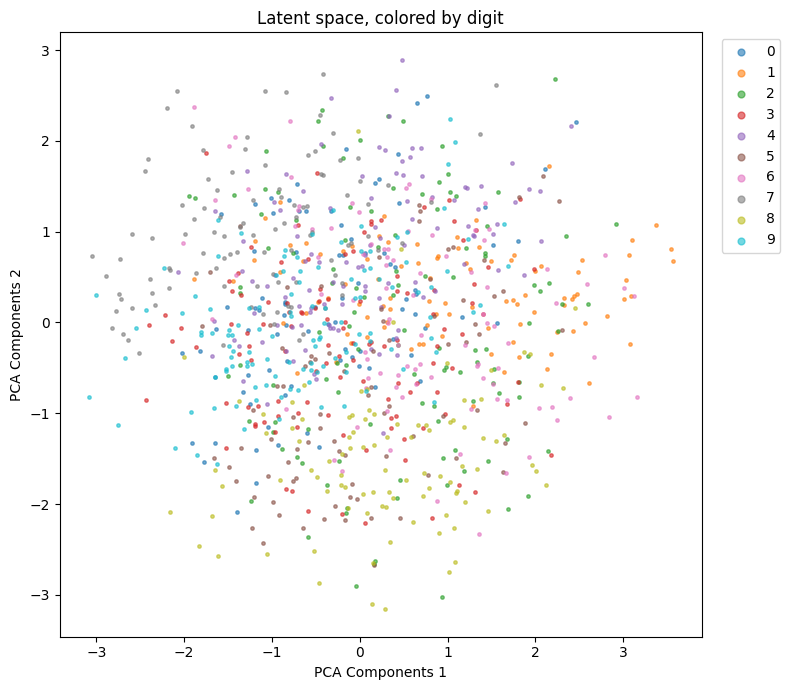
\includegraphics[width=\linewidth]{assets/vae_fig6.png}
\caption{Encoder means $\mu_\phi(x)$ for 1000 training images, reduced to 2D via PCA, colored by digit label, $d=128$.}
\label{fig:vae-pca}
\end{figure}

\begin{figure}[t]
\centering
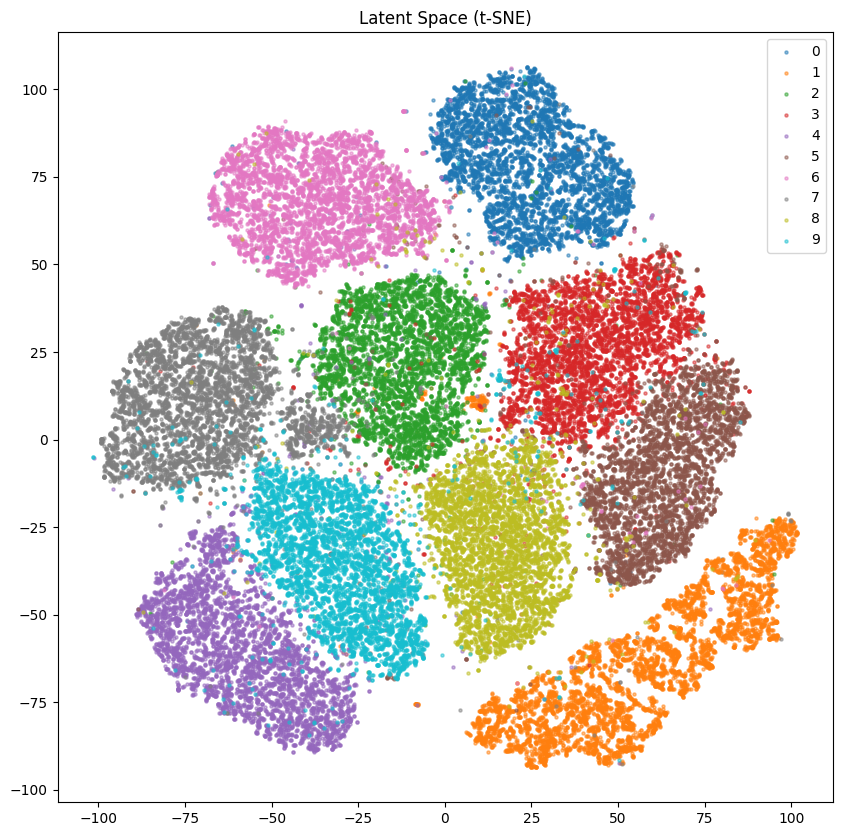
\includegraphics[width=\linewidth]{assets/vae_fig7.png}
\caption{Encoder means $\mu_\phi(x)$ for all 50{,}000 training images, reduced to 2D via t-SNE, colored by digit label, $d=128$.}
\label{fig:vae-tsne}
\end{figure}

The two dimensionality-reduction methods disagree sharply. Under PCA
(Figure~\ref{fig:vae-pca}, 1000 samples), classes are almost completely
intermixed with no visible cluster structure. Under t-SNE
(Figure~\ref{fig:vae-tsne}, all 50{,}000 training samples), the ten classes
form clean, well-separated clusters arranged in a ring, with minimal
cross-class bleeding.

\subsubsection{Effect of Latent Dimensionality: $d=32$ vs.\ $d=128$}

\begin{figure}[t]
\centering
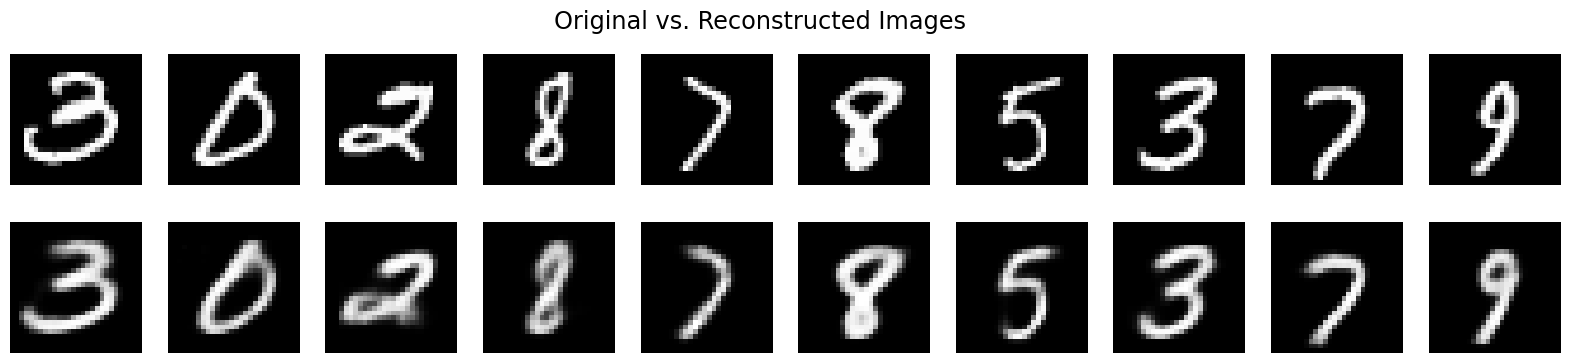
\includegraphics[width=\linewidth]{assets/vae_fig11.png}
\caption{Training-set digits (top row) and reconstructions (bottom row), $d=32$.}
\label{fig:vae-recon-32}
\end{figure}

\begin{figure}[t]
\centering
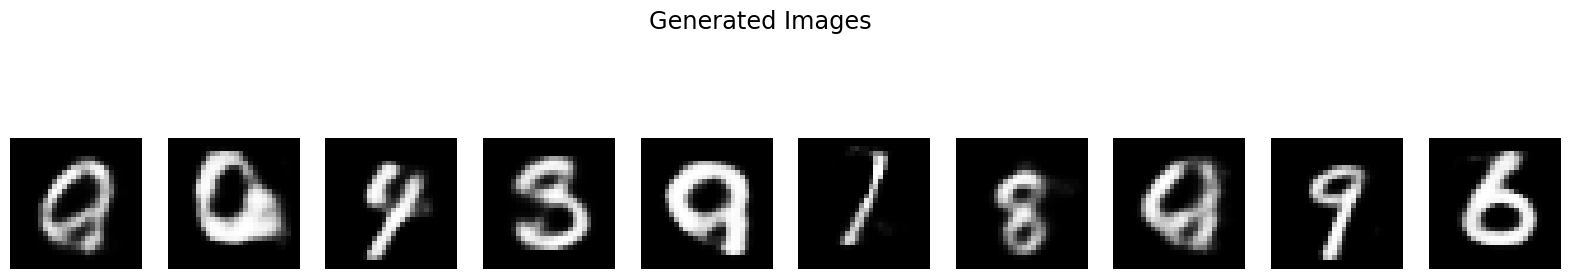
\includegraphics[width=\linewidth]{assets/vae_fig12.png}
\caption{Ten digits generated from the prior, $d=32$.}
\label{fig:vae-gen-32}
\end{figure}

\begin{figure}[t]
\centering
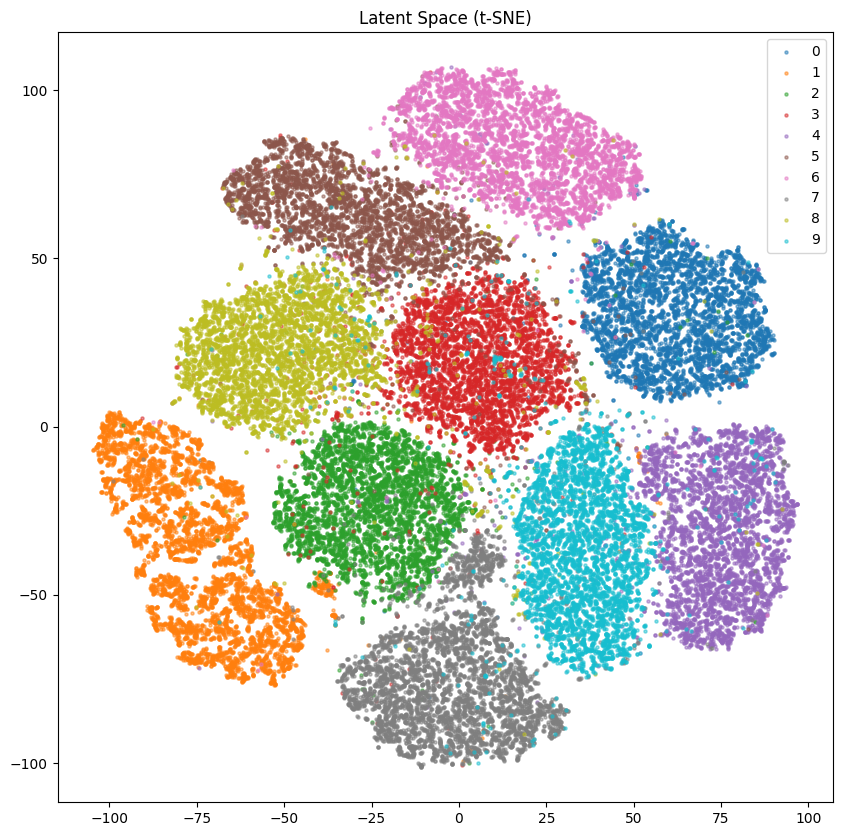
\includegraphics[width=\linewidth]{assets/vae_fig14.png}
\caption{Encoder means, all 50{,}000 training images, t-SNE, $d=32$.}
\label{fig:vae-tsne-32}
\end{figure}

\begin{table}[t]
\centering
\caption{Test-set metrics, $d=128$ vs.\ $d=32$, identical 20-epoch protocol.}
\label{tab:vae-dim-compare}
\begin{tabular}{lcc}
\hline
Metric & $d=128$ & $d=32$ \\
\hline
Total loss (nats) & 104.39 & 103.27 \\
Reconstruction (BCE) & 85.27 & 84.73 \\
KL divergence & 19.12 & 18.54 \\
\hline
\end{tabular}
\end{table}

Table~\ref{tab:vae-dim-compare} shows the $d=32$ model matching, and
marginally exceeding, the $d=128$ model on every test-set metric under an
identical training budget -- reconstruction loss is $0.54$ nats lower and
KL divergence $0.58$ nats lower. The $t$-SNE latent-space visualization at
$d=32$ (Figure~\ref{fig:vae-tsne-32}) shows the same clean, well-separated
ring-of-clusters structure as $d=128$ (Figure~\ref{fig:vae-tsne}), and its
reconstruction grid (Figure~\ref{fig:vae-recon-32}) preserves class
identity on all ten test digits (3,0,2,8,7,8,5,3,7,9) just as the $d=128$
grid does. The one qualitative difference is in generation
(Figure~\ref{fig:vae-gen-32}): more of the ten prior samples at $d=32$
have soft, rounded, blended shapes than at $d=128$, though this is a
subjective visual impression from ten samples, not a measured quantity.

\subsection{Discussion}
\label{sec:vae-discussion}

\subsubsection{Why PCA and t-SNE Disagree on the Latent Space}

PCA finds the two directions of maximum variance in the raw
latent space, $\arg\max_{\|w\|=1}\mathrm{Var}(w^\top z)$ -- a purely linear
criterion with no guarantee that the directions of greatest variance
coincide with the directions along which digit identity varies. In a
high-dimensional space, class-discriminative structure can easily be spread
across dozens of dimensions that individually carry only modest variance,
all of which a 2-component PCA projection will simply miss -- and
Figure~\ref{fig:vae-pca} confirms this holds even at the smaller $d=32$.
t-SNE instead directly optimizes to preserve \emph{local} neighbor
relationships, via a KL divergence between a Gaussian neighbor-similarity
distribution in the original space and a Student-$t$ neighbor-similarity
distribution in 2D -- points close in the original latent space are pulled
close in 2D regardless of which linear directions of the original space
they occupy. The conclusion is that the latent space \emph{is} meaningfully
organized by digit at both dimensionalities tested -- PCA is simply the
wrong lens for this particular space, since the class-separating structure
is not the dominant linear-variance direction.

\subsubsection{Reconstruction Blur is Structural, Not a Defect}

The reconstruction term $-\mathbb{E}_{q(z|x)}[\log p_\theta(x|z)]$ is a
per-pixel-independent Bernoulli log-likelihood: nothing in it rewards
joint, cross-pixel sharpness. Combined with the expectation being taken
over a distribution of $z$ rather than one deterministic code, the
decoder's loss-minimizing behavior in any region of latent space mapping to
more than one plausible stroke pattern is to output the pixel-wise
\emph{average} of those patterns -- averaging several sharp-but-differently
positioned edges is exactly what produces a soft gradient instead of a hard
edge. This is the standard, well-documented explanation for why VAE outputs
are characteristically blurrier than GAN outputs, and is independent of
this particular implementation; an MLP's lack of convolutional locality
bias (relative to a CNN-based VAE) is a secondary, architecture-specific
contributor.

\subsubsection{Generation Quality and the Aggregate Posterior}
\label{sec:vae-discussion-generation}

Reconstruction only exercises the specific regions of latent space the
encoder visits for real images. Generation samples uniformly from the
\emph{entire} prior, so its quality depends on how well the
\textbf{aggregate posterior} $q(z)=\mathbb{E}_x[q(z|x)]$ -- the overall
distribution of codes the encoder actually produces across the dataset --
matches $\mathcal{N}(0,I)$ everywhere, not just where real data happens to
land. That most prior samples in Figure~\ref{fig:vae-gen} decode to
recognizable, diverse digits is evidence the KL term is doing this job
reasonably well: it is exactly this term that prevents the encoder from
mapping real data to a narrow, arbitrarily-placed region of latent space,
which would leave most of the prior's probability mass decoding to
meaningless output. The remaining ambiguous generations are consistent
with $z$ landing between two adjacent clusters in
Figure~\ref{fig:vae-tsne} (e.g.\ the 4/9 boundary), exactly the
"in-between ambiguous digit" phenomenon Doersch's tutorial also reports.

\subsubsection{Comparison with Doersch's VAE Implementation}

Both this implementation and Doersch's (2016) reference use a simple MLP
encoder/decoder for MNIST with a Bernoulli-per-pixel output and
sigmoid-cross-entropy (BCE) reconstruction loss -- an appropriate choice
since MNIST pixel intensities in $[0,1]$ are naturally interpretable as
per-pixel ``ink probability,'' unlike unbounded continuous data, where a
Gaussian/MSE likelihood would be the natural choice instead. Architecturally
this implementation uses a deeper 2-hidden-layer MLP with ReLU activations
($784{\to}512{\to}256{\to}d$ and its mirror) versus Doersch's 1-hidden-layer
MLP with Tanh activations ($784{\to}512{\to}d$ and its mirror); both are
fully-connected, non-convolutional designs.

\textbf{Latent dimensionality.} Doersch reports the VAE's behavior as
largely insensitive to the latent dimensionality across a broad middle
range, degrading only at the extremes ($d$ too small to encode core digit
variation, or so large that gradient optimization becomes impractical).
Table~\ref{tab:vae-dim-compare} tests this directly: $d=32$ and $d=128$
achieve statistically indistinguishable test-set reconstruction loss and
KL divergence under an identical training budget, and both latent spaces
show equally clean class separation under t-SNE
(Figures~\ref{fig:vae-tsne}, \ref{fig:vae-tsne-32}). This is a direct,
measured confirmation of Doersch's insensitivity claim over this
$4\times$ range -- for a dataset as simple as MNIST, the information
needed to reconstruct a digit evidently fits comfortably within 32
dimensions already, so quadrupling the latent budget to 128 buys
essentially no quantitative improvement, only a milder qualitative
impression of cleaner generations (Figure~\ref{fig:vae-gen} vs.\
Figure~\ref{fig:vae-gen-32}) that a 10-sample comparison cannot establish
rigorously. This is consistent with the mechanism Doersch describes:
surplus latent capacity is simply left unused by the encoder (posterior
collapses toward the prior, $\mu_j\approx0,\sigma_j^2\approx1$, on inactive
dimensions) rather than actively harming training.

\textbf{Results comparison.} Doersch's tutorial reports mostly realistic
generated digits with occasional ``in-between'' ambiguous cases; the
generations observed here at both $d=128$ and $d=32$ show the same
qualitative pattern -- a majority of clean, recognizable digits alongside
a minority of blended, boundary-case shapes -- consistent in kind, though
a direct quantitative comparison would require matching Doersch's exact
evaluation protocol.
